\chapter{Introduction}

%-------------------------------------------------------
This assignment demonstrates three different approaches for image segmentation: the twoclass model using Otsu's binarization, Otsu's method with multiple thresholds, and Mean Shift segmentation. A graphic user interface was also built using Tkinter entirely so users could interactively experiment with these segmentation techniques. The function Otsu's Method for Two Classes converts the given image into a grayscale image and uses Otsu's thresholding method from OpenCV. This method automatically calculates the optimal threshold value to separate the image into objects and background. The output from the process on the segmented image is converted into a Tkinter-compatible format. Expanding upon this, Otsu's method for multiple classes extends the thresholding into a more complex process rather than a simple binary partition into two classes. This is made possible by the threshold multiotsu function from skimage.filters. Using the GUI, users may choose how many classes they may want, whereas the segmented regions are given different colors through the use of a Matplotlib colormap for enhanced visual differentiation. The implementation of the Mean Shift Segmentation method is given respect to OpenCV's pyrMeanShiftFiltering method for image clustering based on pixel similarity, taking into account both spatial and chromatic similarity using the spatial radius with the parameter sp and the color range radius with the parameters sr. Overall, this assigment clearly progresses through different image segmentation techniques to demonstrate their effectiveness to separate different regions within the images. The Interactive GUI enhances usability and  enables the user to experiment with various segmentation parameters and thereby instantly observe the changes. %%%%%%%%%%%%%%%%%%%%%%%%%%%%%%%%%%%%%%%%%%%
%%% SUBSECTION NAME
%%%%%%%%%%%%%%%%%%%%%%%%%%%%%%%%%%%%%%%%%%%%%%%%%%%%%

\chapter{Implementation}
\subsection{Explanation Of Tkinter GUI to Usable CV2 Images}
In order to calculate any type of filter or computation on an image and display it using Tkinter we need to convert the CV2 read image into a Tkinter display image. When CV2 reads an image it uses a numPY array to store the values. In order for Tkinter to be able to read and display the image we need to convert its color space from Blue Green Red to Red Green Blue and convert its data type from numPY array to Tkinter photoImage. To facilitate the conversion from numPY array to Tkinter Photoimage we can use the Pillow library, this acts as the intermediate between them.
\begin{minted}[fontsize=\small, linenos, breaklines]{python}
    #convert OpenCV image (BGR) to (RGB) format
    stackConvert1 = cv2.cvtColor(stack1, cv2.COLOR_BGR2RGB)
    stackConvert2 = cv2.cvtColor(stack2, cv2.COLOR_BGR2RGB)
    #convert the initial image to a format for Tkinter after the root window is created
    photo1 = ImageTk.PhotoImage(Image.fromarray(stackConvert1))
    photo2 = ImageTk.PhotoImage(Image.fromarray(stackConvert2))
    #Tkinter display and pac
    imageTop = tk.Label(root, image=photo1)
    imageTop.pack(padx=10, pady=10)
\end{minted}
And the other way as well
\begin{minted}[fontsize=\small, linenos, breaklines]{python}
#convert TKimage to a PIL Image
    image = ImageTk.getimage(image)
    #convert to numpy array
    imageNP = np.array(image)
    #convert color
    imageNP = cv2.cvtColor(imageNP, cv2.COLOR_RGB2BGR)
\end{minted}


\subsection{Explanation Of Tkinter GUI}
For this assignment Tkinter GUI was the best option to be used. It allows all the images and options to be in one window instead of separate ones. Below is the full screenshot of the Tkinter GUI made for this Assignment, the bottom left features two drop boxes. The left one allows you to select what type of Image Segmentation you want to select, between Otsu Method many and 2 classes as well as Mean Shift Segmentation. the right dropbox allows you to select between the photos present in the program - 3. The apply button will apply the Segmentation to the bottom image changing it to reflect the segmentation you selected. The close button will quit out of the app and the reset button will reset the bottom image to the original image. Tkinter only had a slight learning curve compared to using npStack, but it turned out to be a better option because of its look and ease of use with the options we needed.
\begin{figure}[h!]
    \centering
    
\includegraphics[width = .96\textwidth]{figuire1.png}
    \caption[Full Tkinter GUI]%
    {Full Tkinter GUI} 
    \label{fig:exA}
\end{figure}
\begin{figure}[h!]
    \centering
    \begin{minipage}{0.48\textwidth}
        \centering
        
\includegraphics[width=\textwidth]{figuire2.png}
        \caption[Segmentation Dropdown Box]{Segmentation Dropdown Box}
        \label{fig:exB}
    \end{minipage}
    \hfill
    \begin{minipage}{0.48\textwidth}
        \centering
        
\includegraphics[width=\textwidth]{figuire3.png}
        \caption[Image Dropdown]{Image Dropdown}
        \label{fig:exC}
    \end{minipage}
\end{figure}

\begin{minted}[fontsize=\small, linenos, breaklines]{python}
#create tkinter window
root = tk.Tk()
root.title("Assignment 3 App")

imageT = imageB = cv2.imread('Assignment3/Image1.png')
photo1 = ConvertCV2ToTKINTER(imageT)
photo2 = ConvertCV2ToTKINTER(imageB)

#label to display image
imageTop = tk.Label(root, image=photo1)
imageTop.pack(padx=10)
imageBottom = tk.Label(root, image=photo2)
imageBottom.pack(padx=10)

#keeps image refernec so scope dosent destroy it
imageBottom.image = photo2
imageTop.image = photo1

#create a dropdown menu for filter selection
filterCombo = ttk.Combobox(root, values=[
    "Otsu Method (2 Classes)",
    "Otsu Method (Many Classes)",
    "Mean Shift Method"
], state="readonly")

filterCombo.set("Otsu Method (2 Classes)")
filterCombo.pack(side=tk.LEFT, pady=10)
#bind filter selection event
filterCombo.bind("<<ComboboxSelected>>", lambda event: updateGUI())

#dropdown for number of classes (Initially hidden)
classCombo = ttk.Combobox(root, values=[str(i) for i in range(3, 11)], state="readonly")
classCombo.set("3")  # Default to 3 classes

#dropdown for filter dimension
combo = ttk.Combobox(root, values=['Image1', 'Image2' ,'Image3'], state="readonly")
combo.set('Image1')
combo.pack(side = tk.LEFT,pady=10)
combo.bind("<<ComboboxSelected>>", lambda event: changePIC())


#Buttons
applyButton = tk.Button(root, text="Apply", command=applyFilter)
applyButton.pack(side=tk.LEFT, pady=10)
resetButton = tk.Button(root, text="Reset", command=changePIC)
resetButton.pack(side = tk.LEFT, pady=10)
closeButton = tk.Button(root, text="Close", command=root.quit)
closeButton.pack(side = tk.LEFT, pady=10)

#run the Tkinter window
root.mainloop()
\end{minted}

\subsection{Explanation Of Otsu Binary Thresholding}
As we have binary images, the mission of the Otsu's method is to attempt to seek a value of t that will cause the weighted within-class variance expressed by the formula:
\begin{equation}
\sigma_w^2(t) = q_1(t)\sigma_1^2(t)+q_2(t)\sigma_2^2(t)
\end{equation}
\begin{equation}
q_1(t) = \sum_{i=1}^{t} P(i) \quad \& \quad q_2(t) = \sum_{i=t+1}^{I} P(i)
\end{equation}
\begin{equation}
\mu_1(t) = \sum_{i=1}^{t} \frac{iP(i)}{q_1(t)} \quad \& \quad \mu_2(t) = \sum_{i=t+1}^{I} \frac{iP(i)}{q_2(t)}
\end{equation}
\begin{equation}
\sigma_1^2(t) = \sum_{i=1}^{t} [i-\mu_1(t)]^2 \frac{P(i)}{q_1(t)} \quad \& \quad \sigma_2^2(t) = \sum_{i=t+1}^{I} [i-\mu_2(t)]^2 \frac{P(i)}{q_2(t)}
\end{equation}
(See Reference 2)
Otsu Binary (2 class) method will seek out a threshold on the histogram that best seperates the image based on the variance of the frequency of all the pixles. This threshold will then be used as a cut off point. For example if t = 170, any pixel values above 170 will be white and any below 170 will be black, this can be usefull to segment specific types of images. For example image three it works well because the image is less complex and has destinct regions.
\begin{figure}[h!]
    \centering
    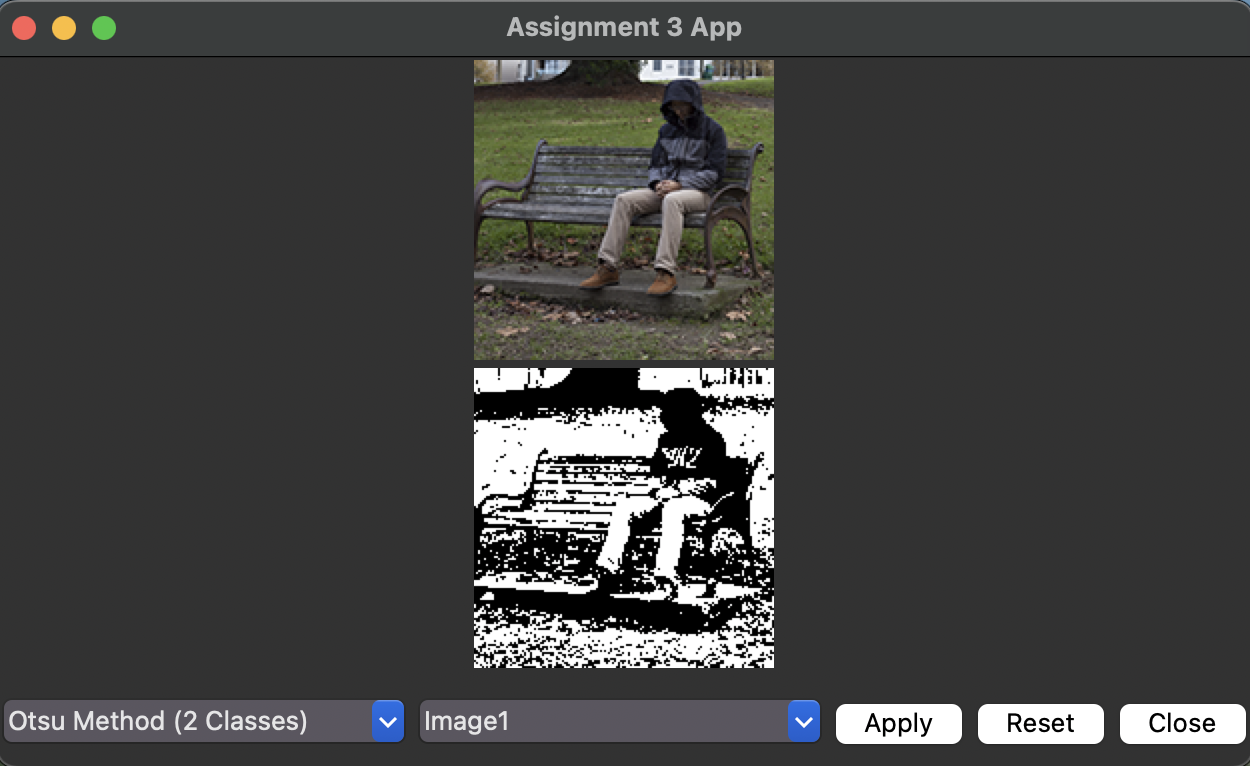
\includegraphics[width = .80\textwidth]{OTSU21.png}
    \caption[Otsu Method (2 Classes) Image 1]%
    {Otsu Method (2 Classes) Image 1} 
    \label{fig:exD}
\end{figure}
\begin{figure}[h!]
    \centering
    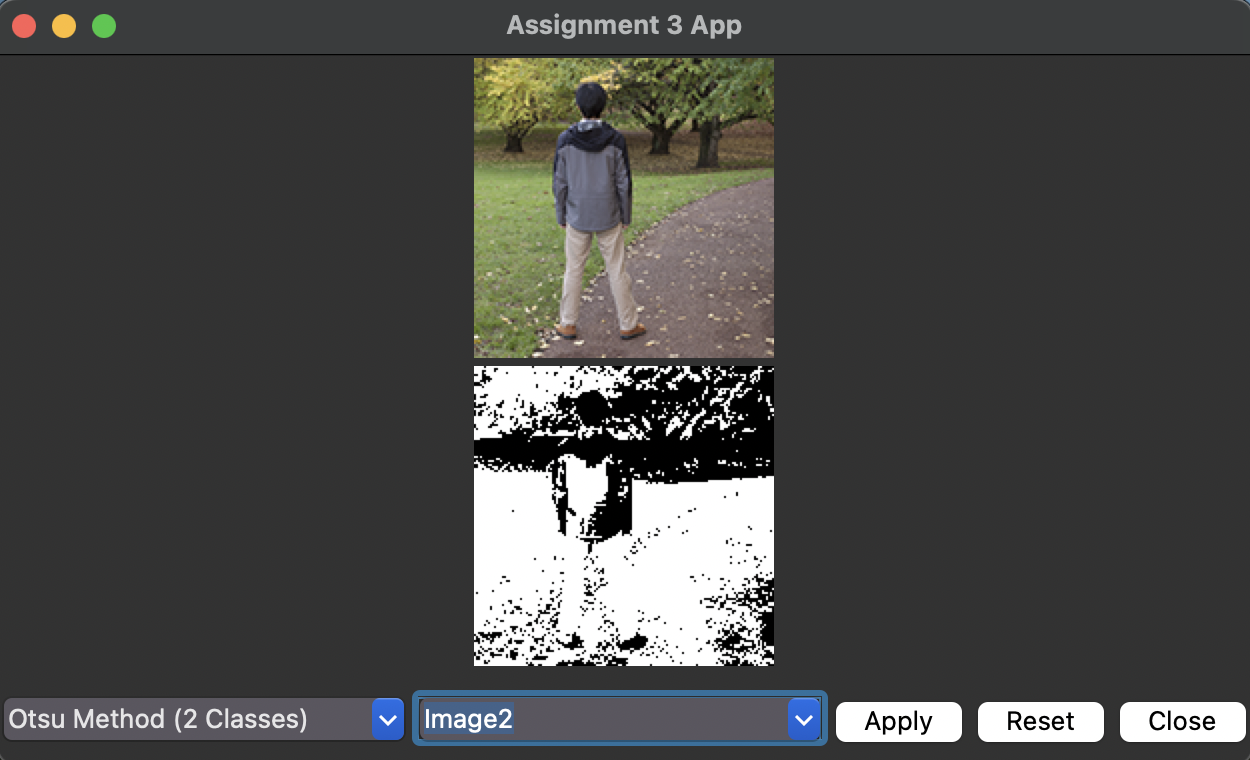
\includegraphics[width = .80\textwidth]{OTSU22.png}
    \caption[Otsu Method (2 Classes) Image 2]%
    {Otsu Method (2 Classes) Image 2} 
    \label{fig:exE}
\end{figure}
\begin{figure}[h!]
    \centering
    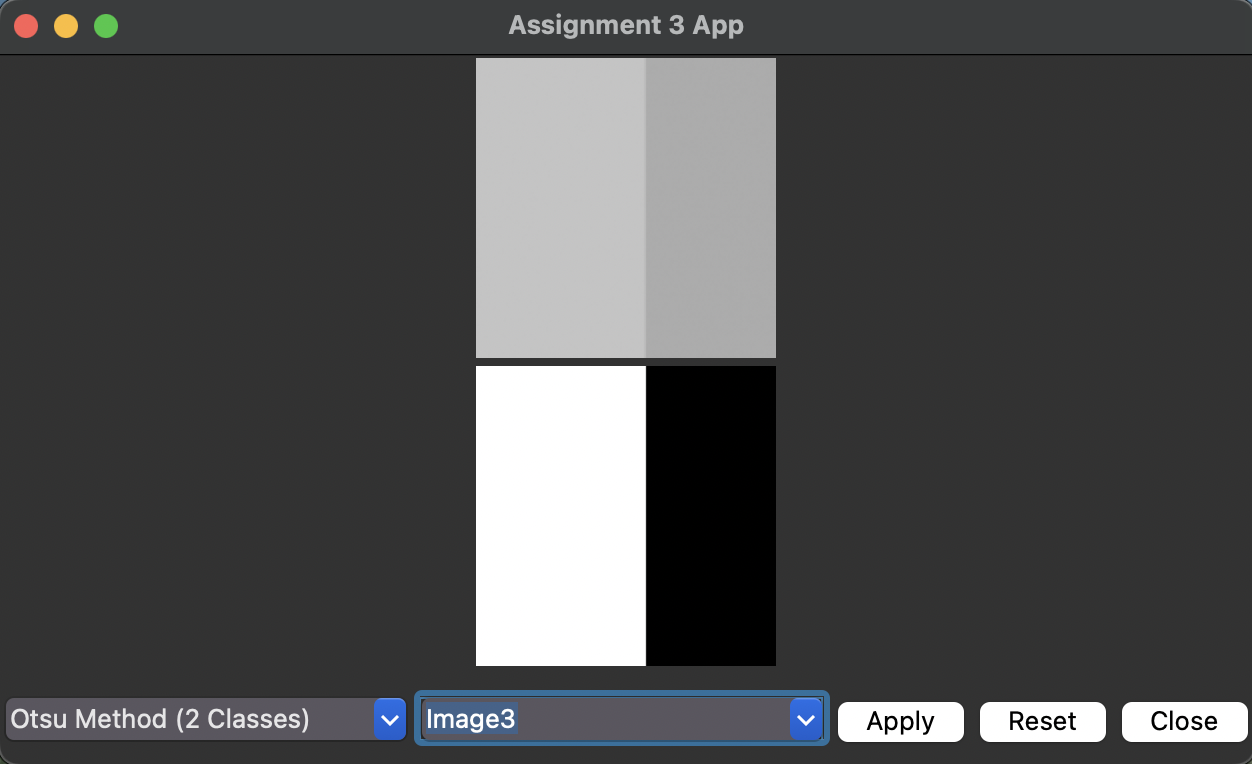
\includegraphics[width = .80\textwidth]{OTSU23.png}
    \caption[Otsu Method (2 Classes) Image 3]%
    {Otsu Method (2 Classes) Image 3} 
    \label{fig:exF}
\end{figure}
\clearpage
Implamentation:
\begin{minted}[fontsize=\small, linenos, breaklines]{python}
def otsu2Classes(image):
    
    imageNP = ConverTKINTERtoCV2(image)
    gray = cv2.cvtColor(imageNP, cv2.COLOR_BGR2GRAY)

    #this function automatically applies and calculates the threshold using cv2 methods
    #the threeshold variable stores the actual value of the threshold
    threshold, filteredImage = cv2.threshold(gray, 0, 255, cv2.THRESH_BINARY + cv2.THRESH_OTSU)

    #convert back to CV2
    filteredImage = ConvertCV2ToTKINTER(filteredImage)

    #update display and image
    imageBottom.config(image=filteredImage)
    imageBottom.image = filteredImage

    return
\end{minted}
\subsection{Explanation Of Otsu Multi-Thresholding}
Otsu Multi-Thresholding is a similar concept to Binary thresholding but instead of picking one threshold it picks mutiple thresholds which can be user defined, these thresholds are calcuated on the same concept as the one threshold, but instead its seprated into a defined amount of classes. Also we used numpys built in color map to map colors to each of the regions.
\begin{minted}[fontsize=\small, linenos, breaklines]{python}
def otsuManyClasses(image):
    imageNP = ConverTKINTERtoCV2(image)
    #make image gray
    gray = cv2.cvtColor(imageNP, cv2.COLOR_BGR2GRAY)

    #we can change the class count here
    classes = int(classCombo.get())

    #qpply Multi-Otsu Thresholding
    thresholds = threshold_multiotsu(gray, classes=classes)

    #assign labels to different regions
    regions = np.digitize(gray, bins=thresholds)

    #convert regions fomr 64 bit to 8 bit for tkinter
    regions = util.img_as_ubyte(regions)

    #generate a colormap based on matplots preset tab10 colorset, so the colors are always distincly different
    #than normalize those color values to scale to grey scale
    colormap = np.array([plt.cm.get_cmap("tab10")(i)[:3] for i in range(classes)]) * 255
    
    #empty image to cast colors to
    color = np.zeros((*gray.shape, 3), dtype=np.uint8)

    #apply colors to each of the regions in the range
    for i in range(classes):
        color[regions == i] = colormap[i]

    #convert back to Tkinter format
    filteredImage = ConvertCV2ToTKINTER(color)

    #update the Tkinter image label
    imageBottom.config(image=filteredImage)

    #keep image reference
    imageBottom.image = filteredImage

    return
\end{minted}
\begin{figure}[h!]
    \centering
    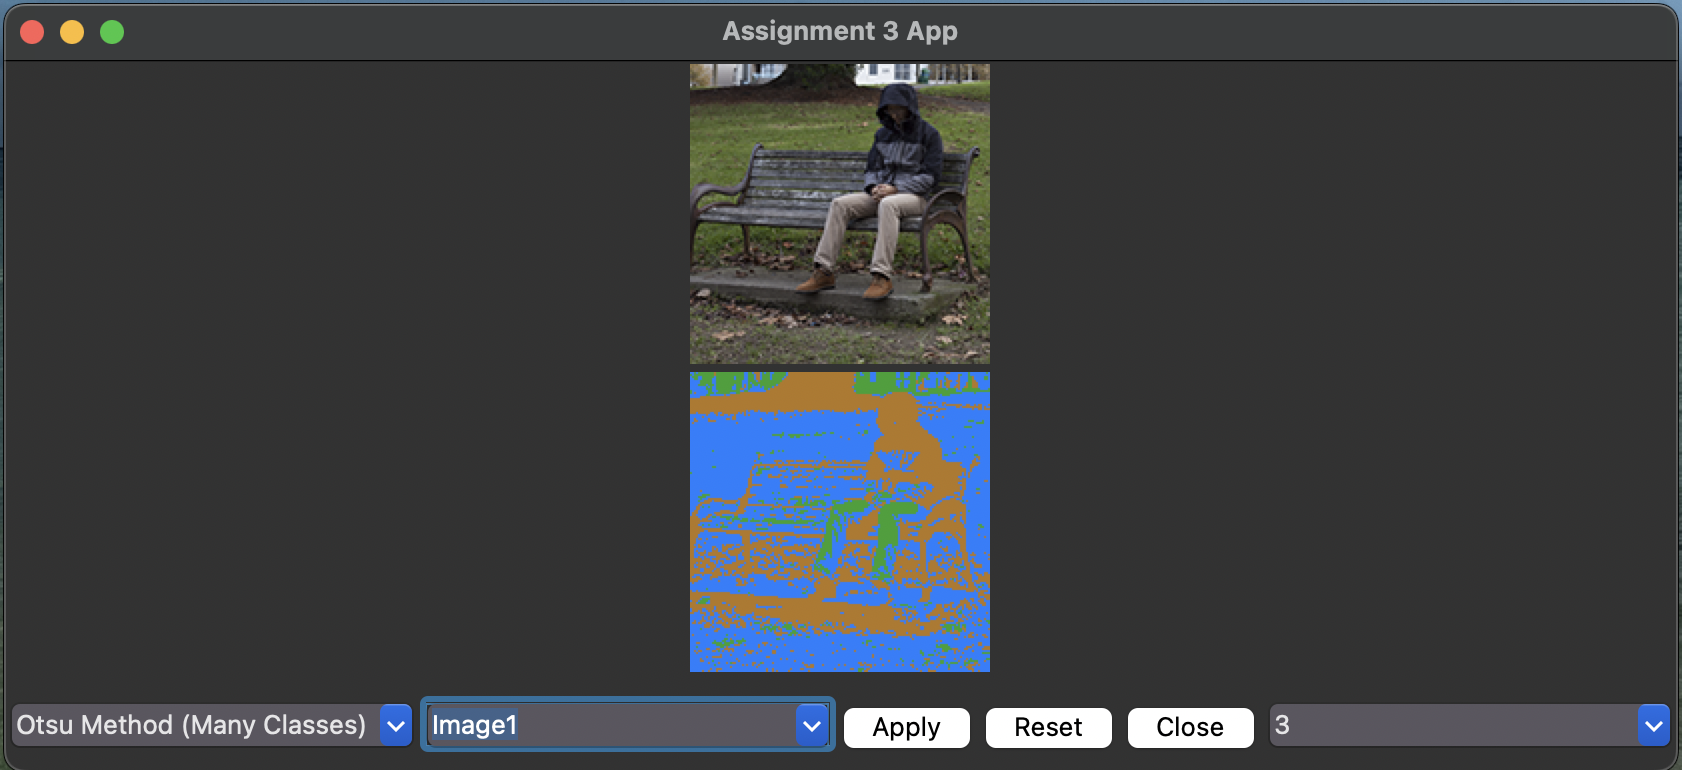
\includegraphics[width = .96\textwidth]{OTSUM1.png}
    \caption[Otsu Method (Three Classes) Image 1]%
    {Otsu Method (Three Classes) Image 1} 
    \label{fig:exG}
\end{figure}
\begin{figure}[h!]
    \centering
    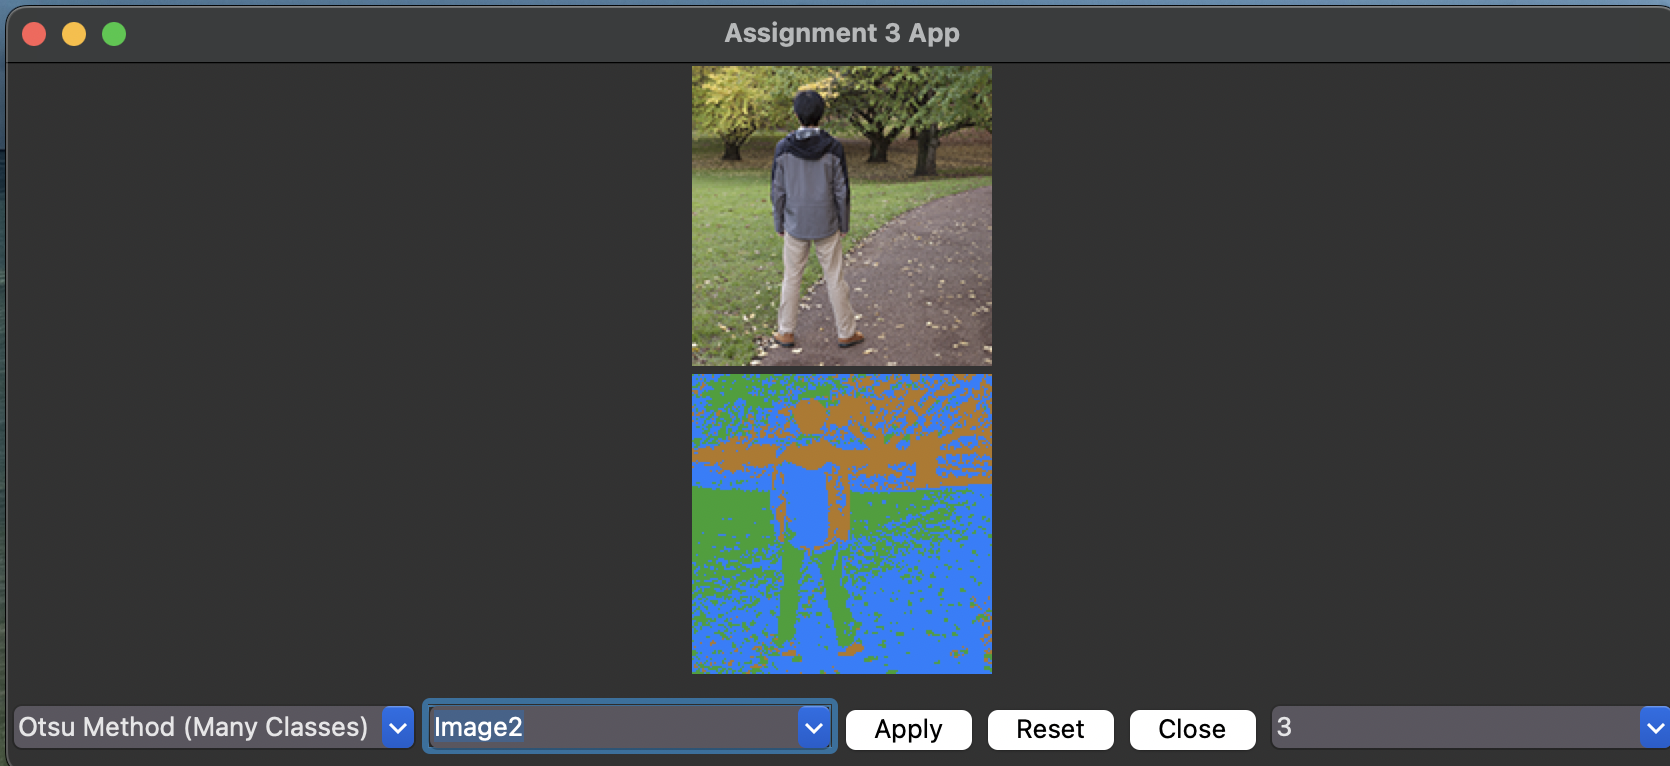
\includegraphics[width = .96\textwidth]{OTSUM2.png}
    \caption[Otsu Method (Three Classes) Image 2]%
    {Otsu Method (Three Classes) Image 2} 
    \label{fig:exH}
\end{figure}
\begin{figure}[h!]
    \centering
    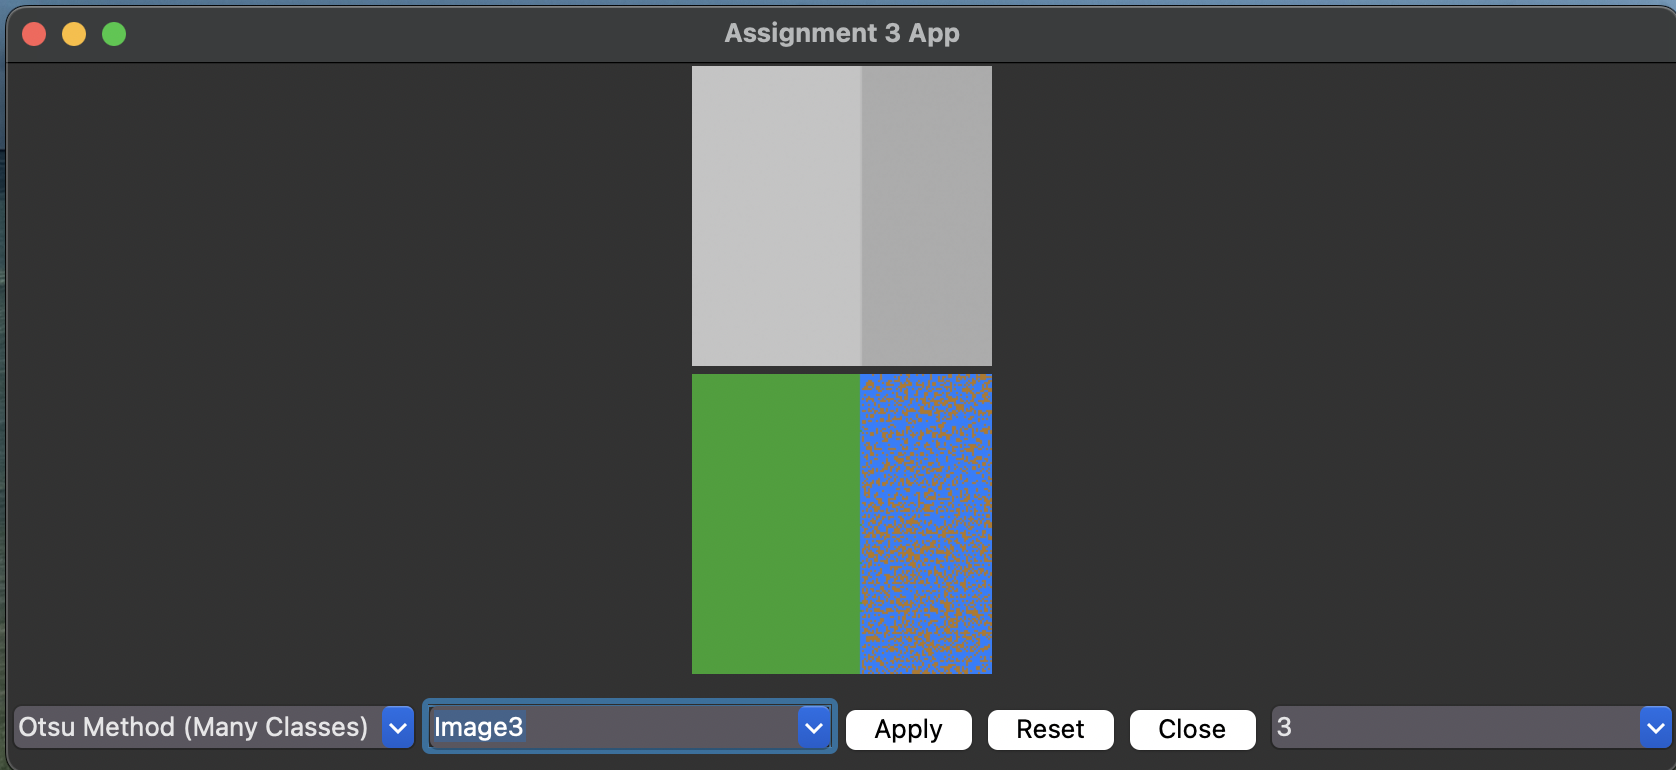
\includegraphics[width = .96\textwidth]{OTSUM3.png}
    \caption[Otsu Method (Three Classes) Image 3]%
    {Otsu Method (Three Classes) Image 3} 
    \label{fig:exI}
\end{figure}
\clearpage
\subsection{Explanation Of Mean Shift Segmentation}
Mean Shift is a clustering-based image segmentation technique that iteratively shifts data points toward the densest regions in the feature space. The steps are as follows:
\begin{enumerate}
    \item Initialize each point $ x $ as a candidate for convergence.
    \item Compute the mean shift vector using the kernel function.
    \item Update the position by shifting the point toward the new mean.
    \item Repeat until convergence (shifts become negligible).
\end{enumerate}
This method was implemented using OpenCV’s pyrMeanShiftFiltering function. This technique clusters pixels based on their spatial and chromatic similarities, controlled by the spatial radius (sp) and color range radius (sr) parameters.
\begin{minted}[fontsize=\small, linenos, breaklines]{python}
    def meanShift(image):
        imageNP = ConverTKINTERtoCV2(image)
    
        """
        sp: Spatial window radius (controls window size).
        sr: Color range radius (controls how similar colors are grouped)
        this line applies meanshift method with the specified permatetors abve
        """
        segmented = cv2.pyrMeanShiftFiltering(imageNP, sp=3, sr=40)
    
        #update image
        filteredImage = ConvertCV2ToTKINTER(segmented)
        imageBottom.config(image=filteredImage)
        imageBottom.image = filteredImage
        return
    \end{minted}
\begin{figure}[h!]
    \centering
    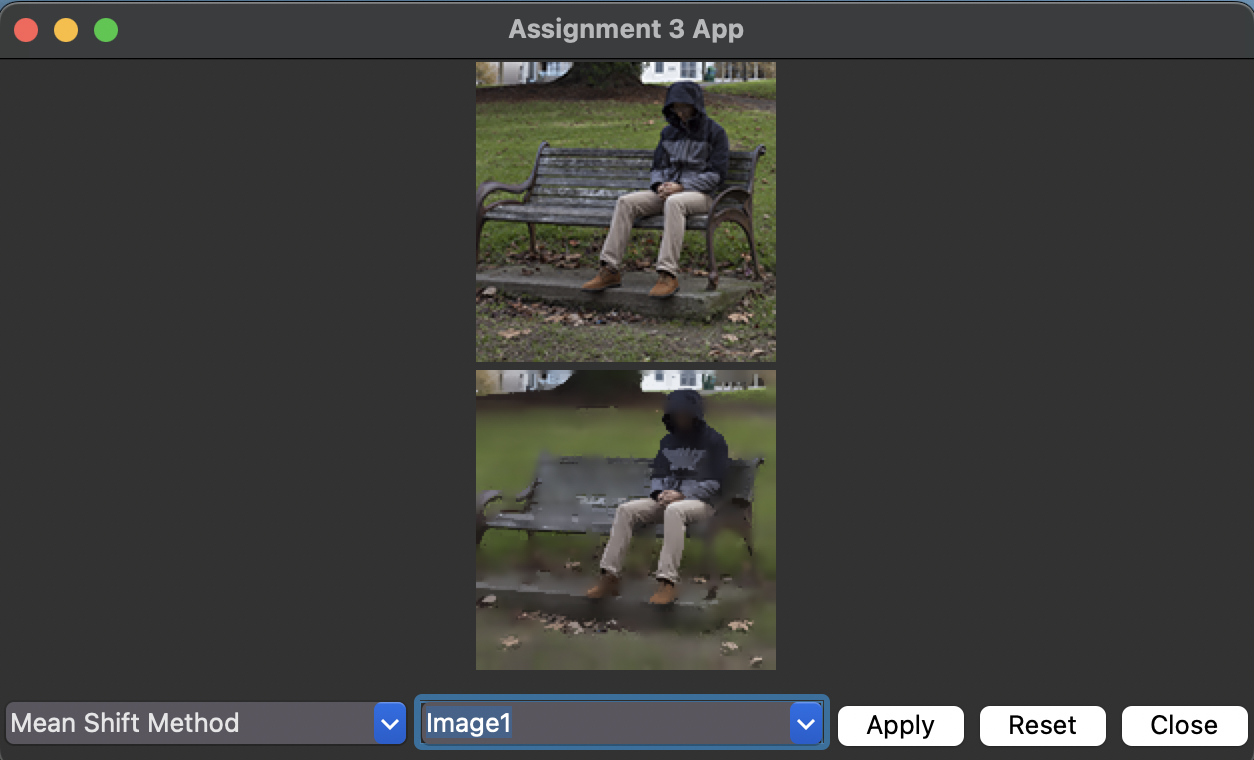
\includegraphics[width = .96\textwidth]{MEAN1.png}
    \caption[Mean Shift Image 1]%
    {Mean Shift Image 1} 
    \label{fig:exK}
\end{figure}
\begin{figure}[h!]
    \centering
    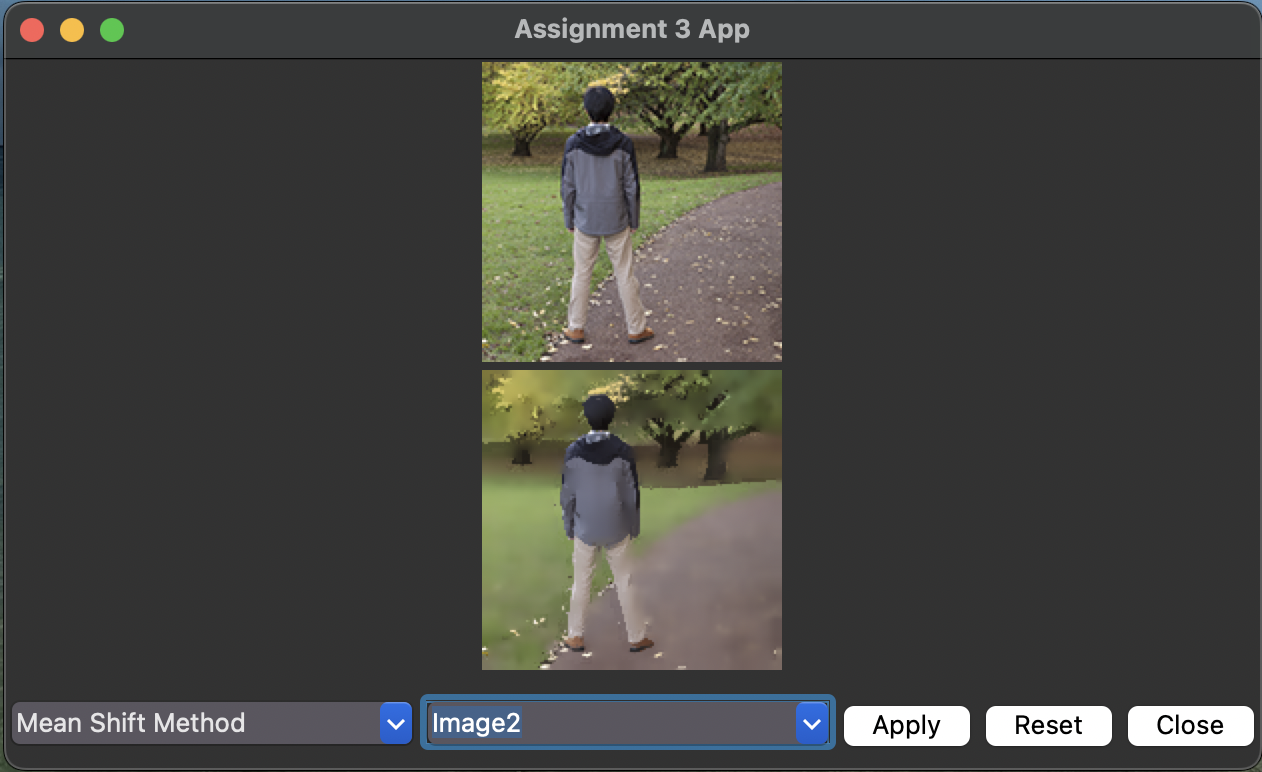
\includegraphics[width = .96\textwidth]{MEAN2.png}
    \caption[Mean Shift Image 2]%
    {Mean Shift Image 2} 
    \label{fig:exL}
\end{figure}
\begin{figure}[h!]
    \centering
    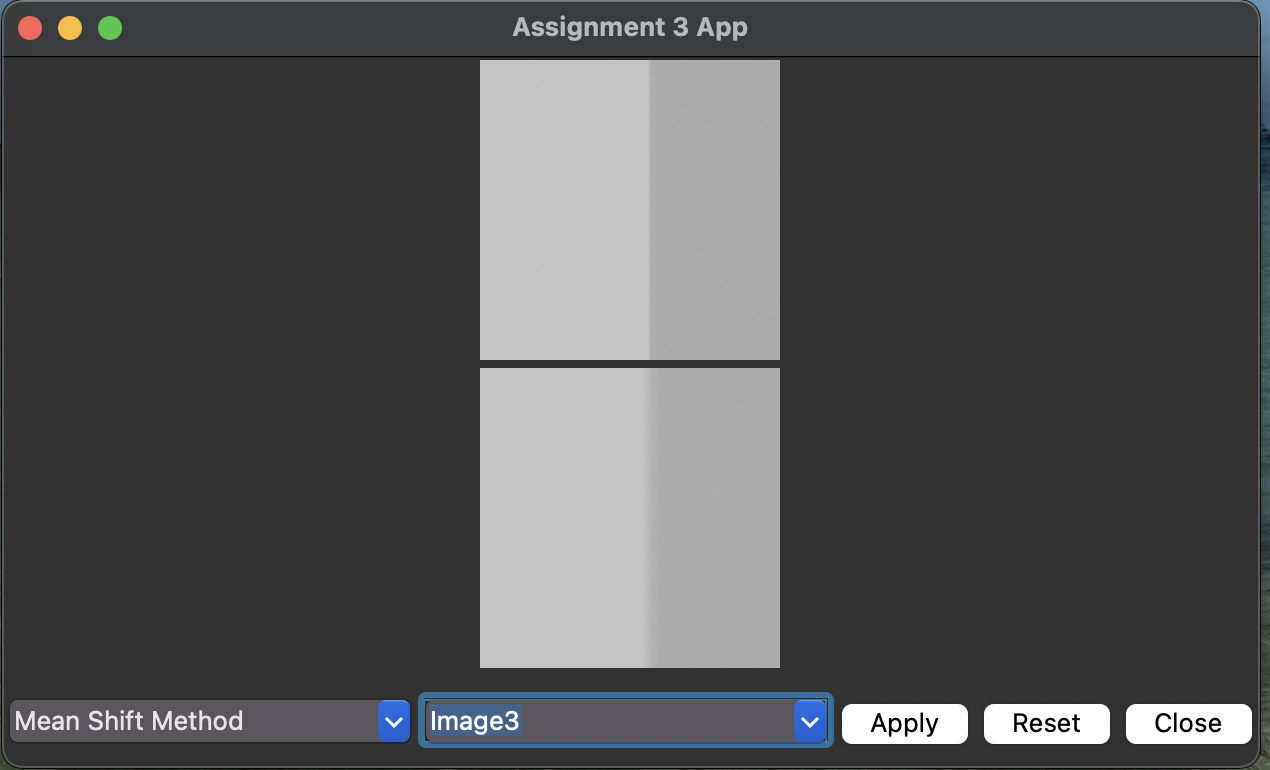
\includegraphics[width = .96\textwidth]{MEAN3.png}
    \caption[Mean Shift Image 3]%
    {Mean Shift Image 3} 
    \label{fig:exM}
\end{figure}
\clearpage
\subsection{Discussion}
I first attempted using Otsu's method on the whole image to determine a global threshold level for segmentation. I soon realized, though, that this was not appropriate since it would not cater to relative light and contrast differences within the different areas of the image. Since we were looking for segmentation of useful areas and not a threshold value for the whole image, we needed a local threshold method. With the use of a local operator, I was able to segment different areas within the image based upon their corresponding intensity distributions adaptively and thus got better region detection. Another problem with the colors used with the segmented areas was that the colors were random and were not facilitating different areas to be differentiated consistently. The colors were most likely resulting from ad hoc color mapping with no structured mapping. The problem was rectified using a colormap offered by NumPy that made color mapping systematic and visually interpretable. The use of a predefined colormap allowed the segmentation results to be better legible and compare the different areas within the image.